\hypertarget{political-views}{%
\chapter{Political Views}\label{political-views}}

This case study explores the relationship between political alignment
(conservative, moderate, or liberal) and other attitudes and beliefs.

In this chapter, we:

\begin{enumerate}
\def\labelenumi{\arabic{enumi}.}
\item
  Explore data from the General Social Survey (GSS), starting with
  political alignment.
\item
  Compare the distribution of responses in 1974 and 1990.
\item
  Plot the mean and standard deviation of responses over time as a way
  of quantifying shifts in political alignment and polarization.
\item
  Use local regression to plot a smooth line through noisy data.
\item
  Use cross tabulation to compute the fraction of respondents in each
  category over time.
\item
  Plot the results using a custom color palette.
\end{enumerate}

As an exercise, you will look at changes in political party affiliation
over the same period.

I've created an HDF file that contains three
\passthrough{\lstinline!DataFrame!} objects with resampled GSS data.
We'll work with the first resampling, \passthrough{\lstinline!gss0!}, to
get started; at the end of this chapter, we'll see the other two as
well.

\begin{lstlisting}[language=Python]
datafile = 'gss_eda.3.hdf5'
gss = pd.read_hdf(datafile, 'gss0')
gss.shape
\end{lstlisting}

\begin{lstlisting}[]
(64814, 169)
\end{lstlisting}

\hypertarget{political-alignment}{%
\section{Political alignment}\label{political-alignment}}

The people surveyed as part of the GSS were asked about their
``political alignment'', which is where they place themselves on a
spectrum from liberal to conservative.

The variable \passthrough{\lstinline!polviews!} contains responses to
the following question (see
\url{https://gssdataexplorer.norc.org/projects/52787/variables/178/vshow}):

\begin{quote}
We hear a lot of talk these days about liberals and conservatives. I'm
going to show you a seven-point scale on which the political views that
people might hold are arranged from extremely liberal--point 1--to
extremely conservative--point 7. Where would you place yourself on this
scale?
\end{quote}

Here are the valid responses:

\begin{lstlisting}[]
1   Extremely liberal
2   Liberal
3   Slightly liberal
4   Moderate
5   Slightly conservative
6   Conservative
7   Extremely conservative
\end{lstlisting}

To see how the responses have changed over time, we'll inspect them at
the beginning and end of the observation period. First I'll select the
column.

\begin{lstlisting}[language=Python]
polviews = gss['polviews']
\end{lstlisting}

Then compute a Boolean Series that's \passthrough{\lstinline!True!} for
responses from 1974.

\begin{lstlisting}[language=Python]
year74 = (gss['year'] == 1974)
\end{lstlisting}

Now we can select the responses from 1974.

\begin{lstlisting}[language=Python]
polviews74 = polviews[year74]
\end{lstlisting}

We'll use the following function to count the number of times each
response occurs.

\begin{lstlisting}[language=Python]
def values(series):
    """Count the values and sort.
    
    series: pd.Series
    
    returns: series mapping from values to frequencies
    """
    return series.value_counts().sort_index()
\end{lstlisting}

Here are the responses from 1974.

\begin{lstlisting}[language=Python]
values(polviews74)
\end{lstlisting}

\begin{tabular}{lr}
\toprule
{} &  polviews \\
\midrule
1.0 &        31 \\
2.0 &       201 \\
3.0 &       211 \\
4.0 &       538 \\
5.0 &       223 \\
6.0 &       181 \\
7.0 &        30 \\
\bottomrule
\end{tabular}

And here are the responses from 2018.

\begin{lstlisting}[language=Python]
year18 = (gss['year'] == 2018)
polviews18 = polviews[year18]
values(polviews18)
\end{lstlisting}

\begin{tabular}{lr}
\toprule
{} &  polviews \\
\midrule
1.0 &        89 \\
2.0 &       269 \\
3.0 &       265 \\
4.0 &       891 \\
5.0 &       310 \\
6.0 &       342 \\
7.0 &        92 \\
\bottomrule
\end{tabular}

\hypertarget{pmfs}{%
\section{PMFs}\label{pmfs}}

To visualize these distributions, we'll use a Probability Mass Function
(PMF), which is similar to a histogram. The difference is that the PMF
is normalized, which means that it shows the fraction of people who gave
each response, rather than the number.

I'll use the \passthrough{\lstinline!Pmf!} class from
\passthrough{\lstinline!empiricaldist!} to compute it.

\begin{lstlisting}[language=Python]
from empiricaldist import Pmf
\end{lstlisting}

Here's the distribution from 1974:

\begin{lstlisting}[language=Python]
pmf74 = Pmf.from_seq(polviews74)
pmf74.bar(label='1974', color='C0', alpha=0.7)

decorate(xlabel='Political view on a 7-point scale',
         ylabel='Fraction of population',
         title='Distribution of political views')
\end{lstlisting}

\begin{center}
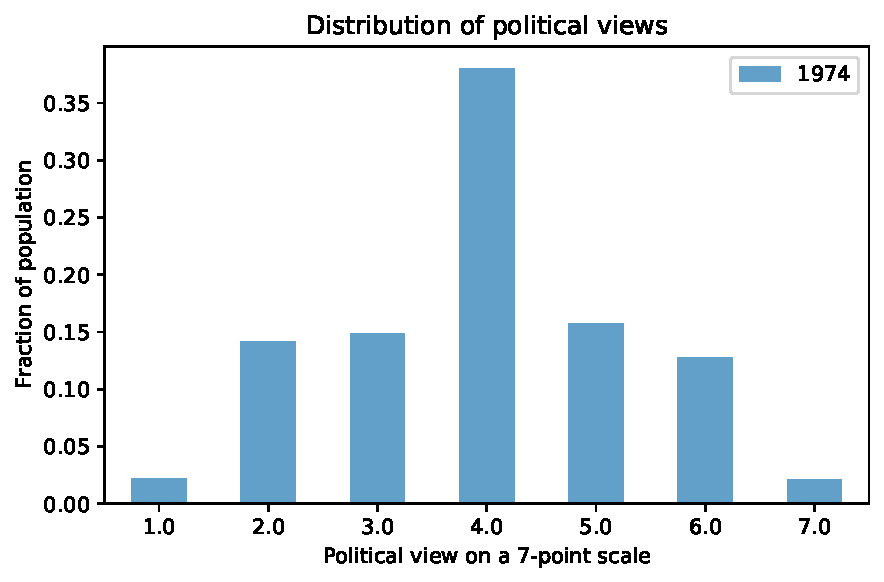
\includegraphics[scale=0.75]{chapters/02_polviews_soln_files/02_polviews_soln_32_0.pdf}
\end{center}

And from 2018:

\begin{lstlisting}[language=Python]
pmf18 = Pmf.from_seq(polviews18)
pmf18.bar(label='2018', color='C1', alpha=0.7)

decorate(xlabel='Political view on a 7-point scale',
         ylabel='Fraction of population',
         title='Distribution of political views')
\end{lstlisting}

\begin{center}
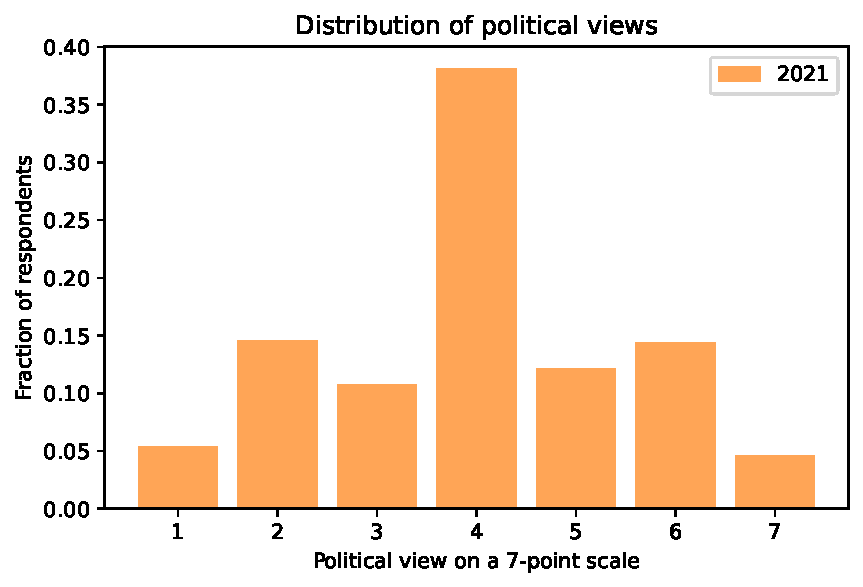
\includegraphics[scale=0.75]{chapters/02_polviews_soln_files/02_polviews_soln_34_0.pdf}
\end{center}

In both cases, the most common response is \passthrough{\lstinline!4!},
which is the code for ``moderate''. Few respondents describe themselves
as ``extremely'' liberal or conservative. So maybe we're not so
polarized after all.

\textbf{Exercise:} To summarize these changes, we can compare the mean
and standard deviation of \passthrough{\lstinline!polviews!} in 1974 and
2018.

The mean of the responses measures the balance of people in the
population with liberal or conservative leanings. If the mean increases
over time, that might indicate a shift in the population toward
conservatism.

The standard deviation measures the dispersion of views in the
population; if it increases over time, that might indicate an increase
in polarization.

Compute the mean and standard deviation of
\passthrough{\lstinline!polviews74!} and
\passthrough{\lstinline!polviews18!}.

What do they indicate about changes over this interval?

\hypertarget{time-series}{%
\section{Time Series}\label{time-series}}

At this point we have looked at the endpoints, 1974 and 2018, but we
don't know what happened in between. To see how the distribution changes
over time, we can group by year and compute the mean of
\passthrough{\lstinline!polviews!} during each year. First I'll use
\passthrough{\lstinline!groupby!} to group the respondents by year.

\begin{lstlisting}[language=Python]
gss_by_year = gss.groupby('year')
gss_by_year
\end{lstlisting}

\begin{lstlisting}[]
<pandas.core.groupby.generic.DataFrameGroupBy object at 0x7fa857dd8e10>
\end{lstlisting}

The result is a \passthrough{\lstinline!DataFrameGroupBy!} object that
represents a collection of groups.

In many ways the \passthrough{\lstinline!DataFrameGroupBy!} behaves like
a \passthrough{\lstinline!DataFrame!}. We can use the bracket operator
to select a column:

\begin{lstlisting}[language=Python]
polviews_by_year = gss_by_year['polviews']
polviews_by_year
\end{lstlisting}

\begin{lstlisting}[]
<pandas.core.groupby.generic.SeriesGroupBy object at 0x7fa8558a9050>
\end{lstlisting}

A column from a \passthrough{\lstinline!DataFrameGroupBy!} is a
\passthrough{\lstinline!SeriesGroupBy!}. If we invoke
\passthrough{\lstinline!mean!} on it, the results is a series that
contains the mean of \passthrough{\lstinline!polviews!} for each year of
the survey.

\begin{lstlisting}[language=Python]
mean_series = polviews_by_year.mean()
\end{lstlisting}

And here's what it looks like.

\begin{lstlisting}[language=Python]
mean_series.plot(color='C2', label='polviews')
decorate(xlabel='Year', 
         ylabel='Mean (7 point scale)',
         title='Mean of polviews')
\end{lstlisting}

\begin{center}
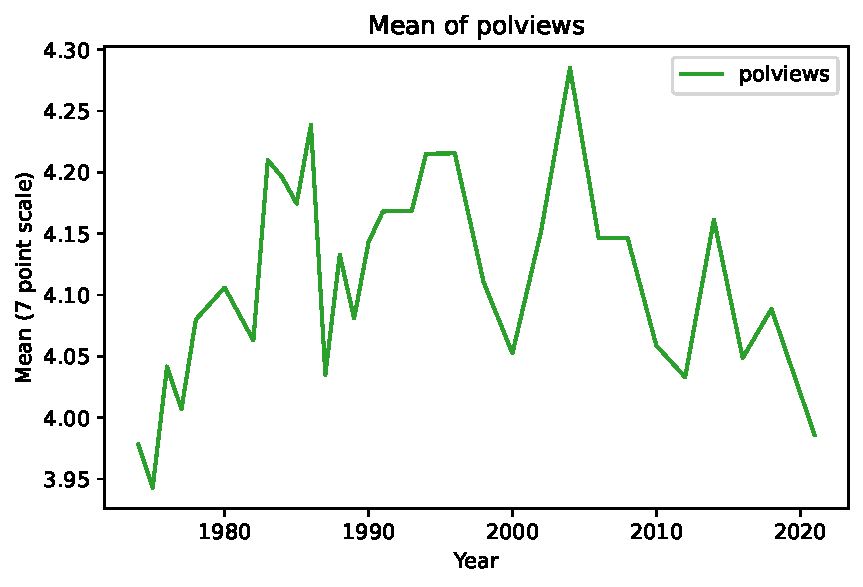
\includegraphics[scale=0.75]{chapters/02_polviews_soln_files/02_polviews_soln_50_0.pdf}
\end{center}

\textbf{Exercise:} The standard deviation quantifies the spread of the
distribution, which is one way to measure polarization. Plot standard
deviation of \passthrough{\lstinline!polviews!} for each year of the
survey from 1972 to 2018. Does it show evidence of increasing
polarization?

\hypertarget{local-regression}{%
\section{Local Regression}\label{local-regression}}

In the previous section we plotted mean and standard deviation of
\passthrough{\lstinline!polviews!} over time. Both plots are quite
noisy. We can use \textbf{local regression} to compute a smooth line
through these data points (see
\url{https://en.wikipedia.org/wiki/Local_regression}).

The following function takes a Pandas Series and uses an algorithm
called LOWESS to compute a smooth line. LOWESS stands for ``locally
weighted scatterplot smoothing''.

\begin{lstlisting}[language=Python]
from statsmodels.nonparametric.smoothers_lowess import lowess

def make_lowess(series):
    """Use LOWESS to compute a smooth line.
    
    series: pd.Series
    
    returns: pd.Series
    """
    y = series.values
    x = series.index.values

    smooth = lowess(y, x)
    index, data = np.transpose(smooth)

    return pd.Series(data, index=index) 
\end{lstlisting}

We'll use the following function to plot data points and the smoothed
line.

\begin{lstlisting}[language=Python]
def plot_series_lowess(series, color):
    """Plots a series of data points and a smooth line.
    
    series: pd.Series
    color: string or tuple
    """
    series.plot(linewidth=0, marker='o', color=color, alpha=0.5)
    smooth = make_lowess(series)
    smooth.plot(label='', color=color)
\end{lstlisting}

The following figure shows the mean of
\passthrough{\lstinline!polviews!} and a smooth line.

\begin{lstlisting}[language=Python]
mean_series = gss_by_year['polviews'].mean()
plot_series_lowess(mean_series, 'C2')
decorate(ylabel='Mean (7 point scale)',
         title='Mean of polviews',
         xlabel='Year',
         xlim=[1972, 2020])
\end{lstlisting}

\begin{center}
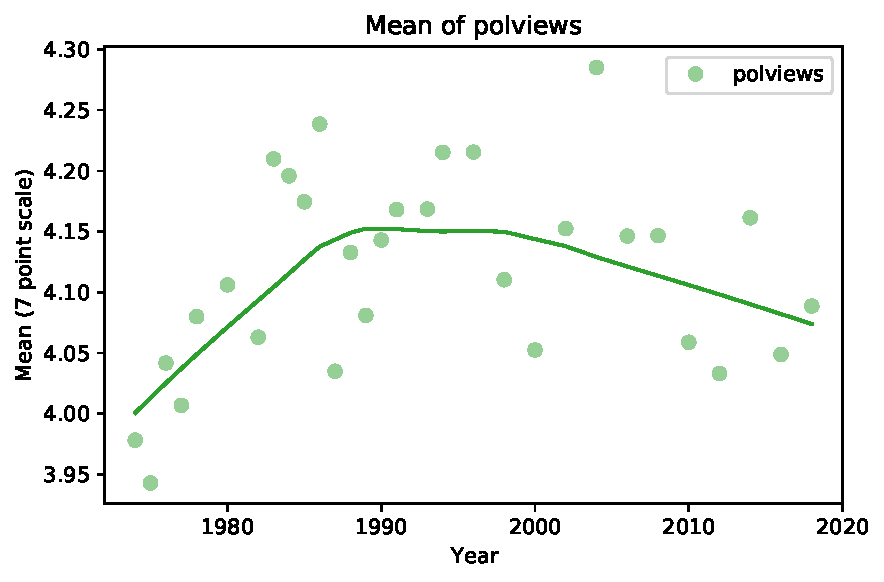
\includegraphics[scale=0.75]{chapters/02_polviews_soln_files/02_polviews_soln_57_0.pdf}
\end{center}

One reason the PMFs for 1974 and 2018 did not look very different is
that the mean seems to have gone up (more conservative) and then down
again (more liberal). Generally, it looks like the U.S. has been
trending toward liberal for the last 20 years, or more, at least in the
sense of how people describe themselves.

\textbf{Exercise:} Use \passthrough{\lstinline!plot\_series\_lowess!} to
plot the standard deviation of \passthrough{\lstinline!polviews!} with a
smooth line.

\hypertarget{cross-tabulation}{%
\section{Cross Tabulation}\label{cross-tabulation}}

In the previous sections, we treated \passthrough{\lstinline!polviews!}
as a numerical quantity, so we were able to compute means and standard
deviations. But the responses are really categorical, which means that
each value represents a discrete category, like ``liberal'' or
``conservative''.\\
In this section, we'll treat \passthrough{\lstinline!polviews!} as a
categorical variable. Specifically, we'll compute the number of
respondents in each category for each year, and plot changes over time.

Pandas provides a function called \passthrough{\lstinline!crosstab!}
that computes a \textbf{cross tabulation} (see
\url{https://en.wikipedia.org/wiki/Contingency_table}). It takes two
\passthrough{\lstinline!Series!} objects as arguments and returns a
\passthrough{\lstinline!DataFrame!}.

\begin{lstlisting}[language=Python]
year = gss['year']
column = gss['polviews']

xtab = pd.crosstab(year, column)
\end{lstlisting}

Here are the first few lines from the result.

\begin{lstlisting}[language=Python]
xtab.head()
\end{lstlisting}

\begin{tabular}{lrrrrrrr}
\toprule
polviews &  1.0 &  2.0 &  3.0 &  4.0 &  5.0 &  6.0 &  7.0 \\
year &      &      &      &      &      &      &      \\
\midrule
1974 &   31 &  201 &  211 &  538 &  223 &  181 &   30 \\
1975 &   56 &  184 &  207 &  540 &  204 &  162 &   45 \\
1976 &   31 &  198 &  175 &  564 &  209 &  206 &   34 \\
1977 &   37 &  181 &  214 &  594 &  243 &  164 &   42 \\
1978 &   21 &  140 &  255 &  559 &  265 &  187 &   25 \\
\bottomrule
\end{tabular}

It contains one row for each value of \passthrough{\lstinline!year!} and
one column for each value of \passthrough{\lstinline!polviews!}. Reading
the first row, we see that in 1974, 31 people gave response 1,
``extremely liberal'', 201 people gave response 2, ``liberal'', and so
on.

The number of respondents varies from year to year, so we need to
normalize the results, which means computing for each year the
\emph{fraction} of respondents in each category, rather than the count.

\passthrough{\lstinline!crosstab!} takes an optional argument that
normalizes each row.

\begin{lstlisting}[language=Python]
xtab_norm = pd.crosstab(year, column, normalize='index')
\end{lstlisting}

Here's what that looks like for the 7-point scale.

\begin{lstlisting}[language=Python]
xtab_norm.head()
\end{lstlisting}

\begin{tabular}{lrrrrrrr}
\toprule
polviews &       1.0 &       2.0 &       3.0 &       4.0 &       5.0 &       6.0 &       7.0 \\
year &           &           &           &           &           &           &           \\
\midrule
1974 &  0.021908 &  0.142049 &  0.149117 &  0.380212 &  0.157597 &  0.127915 &  0.021201 \\
1975 &  0.040057 &  0.131617 &  0.148069 &  0.386266 &  0.145923 &  0.115880 &  0.032189 \\
1976 &  0.021877 &  0.139732 &  0.123500 &  0.398024 &  0.147495 &  0.145378 &  0.023994 \\
1977 &  0.025085 &  0.122712 &  0.145085 &  0.402712 &  0.164746 &  0.111186 &  0.028475 \\
1978 &  0.014463 &  0.096419 &  0.175620 &  0.384986 &  0.182507 &  0.128788 &  0.017218 \\
\bottomrule
\end{tabular}

\hypertarget{plotting}{%
\section{Plotting}\label{plotting}}

To plot the results, I use the following function, which takes a
\passthrough{\lstinline!DataFrame!} and plots each column using
\passthrough{\lstinline!plot\_series\_lowess!}.

\begin{lstlisting}[language=Python]
def plot_columns_lowess(table, columns, colors):
    """Plot the columns in a DataFrame.
    
    table: DataFrame with a cross tabulation
    columns: list of column names, in the desired order
    colors: mapping from column names to colors
    """
    for col in columns:
        series = table[col]
        plot_series_lowess(series, colors[col])
\end{lstlisting}

Here are the 7 categories plotted as a function of time.

\begin{lstlisting}[language=Python]
plot_columns_lowess(xtab_norm, columns, color_map)
decorate(xlabel='Year',
         ylabel='Proportion',
         title='Fraction of people with each political view',
         xlim=[1972, 2020])

anchor_legend(1.02, 1.02)
\end{lstlisting}

\begin{center}
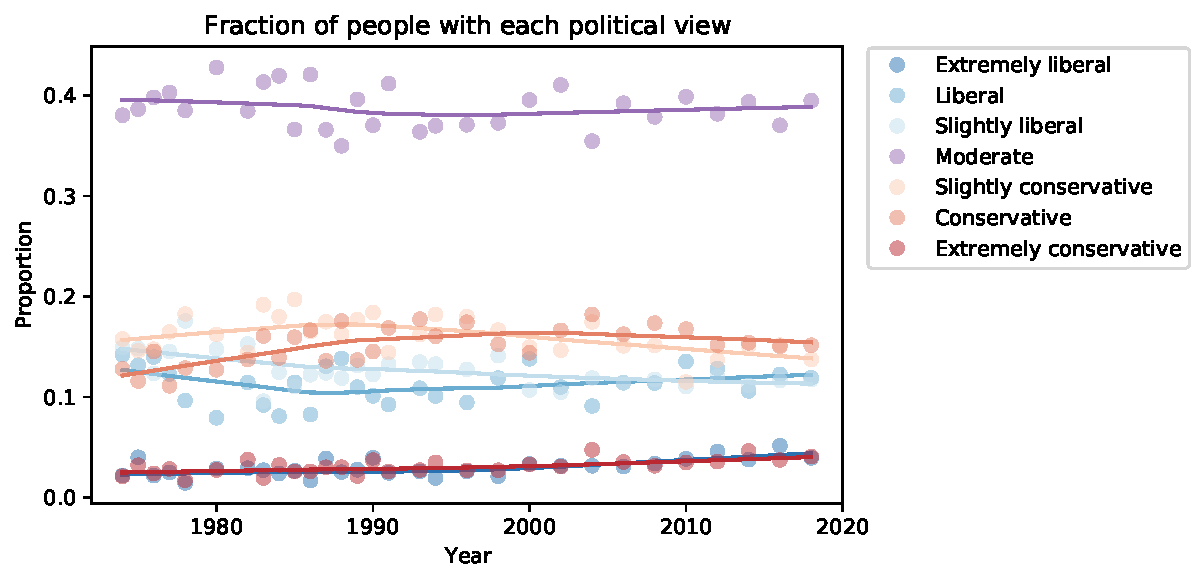
\includegraphics[scale=0.75]{chapters/02_polviews_soln_files/02_polviews_soln_91_0.pdf}
\end{center}

This way of looking at the results suggests that changes in political
alignment during this period have generally been slow and small. The
fraction of self-described moderates has not changed substantially. The
fraction of conservatives increased, but seems to be decreasing now; the
number of liberals seems to be increasing.

The fraction of people at the extremes has increased, but it is hard to
see clearly in this figure. We can get a better view by plotting just
the extremes.

\begin{lstlisting}[language=Python]
columns2 = ['Extremely liberal', 'Extremely conservative']

plot_columns_lowess(xtab_norm, columns2, color_map)
decorate(xlabel='Year',
         ylabel='Proportion',
         title='Fraction of people with extreme political views',
         xlim=[1970, 2020])

anchor_legend(1.02, 1.02)
\end{lstlisting}

\begin{center}
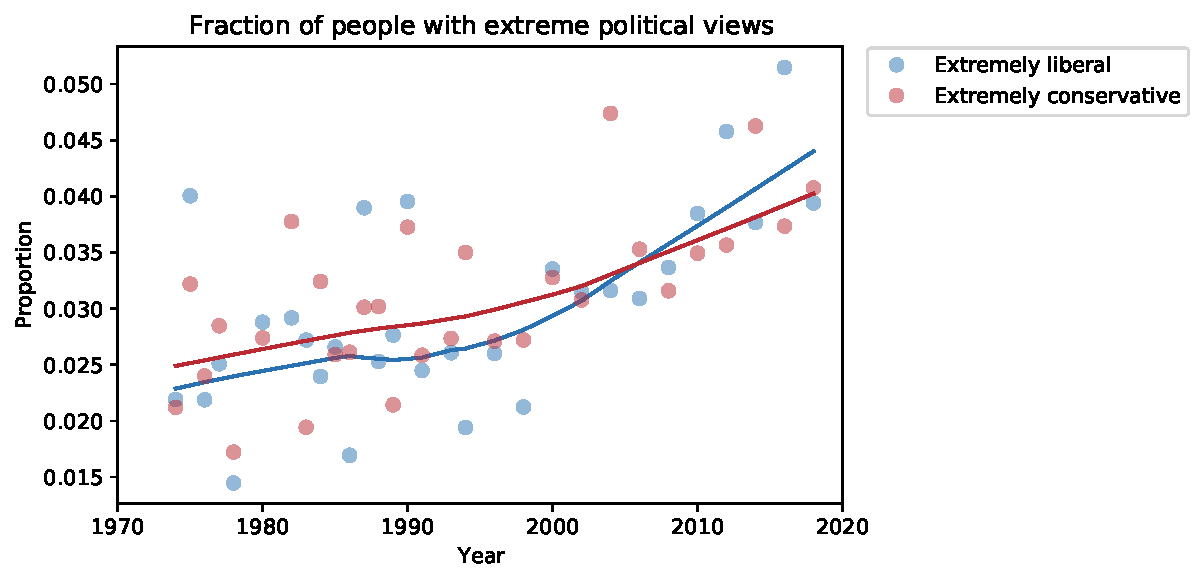
\includegraphics[scale=0.75]{chapters/02_polviews_soln_files/02_polviews_soln_93_0.pdf}
\end{center}

This figure shows that the fraction of people who describe themselves as
``extreme'' has increased from about 2.5\% to about 4\%. In relative
terms, that's a big increase. But in absolute terms these tails of the
distribution are still small.

\textbf{Exercise:} Let's do a similar analysis with
\passthrough{\lstinline!partyid!}, which encodes responses to the
question:

\begin{quote}
Generally speaking, do you usually think of yourself as a Republican,
Democrat, Independent, or what?
\end{quote}

The valid responses are:

\begin{lstlisting}[]
0   Strong democrat
1   Not str democrat
2   Ind,near dem
3   Independent
4   Ind,near rep
5   Not str republican
6   Strong republican
7   Other party
\end{lstlisting}

You can read the codebook for \passthrough{\lstinline!partyid!} at
\url{https://gssdataexplorer.norc.org/projects/52787/variables/141/vshow}.

